\begin{table}[tbp]
\caption{Summary of benchmark settings.}
\label{Table: Benchmark Settings}\centering
\begin{tabular}{ll}
\hline\hline
Agent           & Totals\\
\hline
Regions         & 1\\
\hline
Household       & 1600\\
Firm            & 80\\
IGFirm          & 1\\
Mall            & 1\\
Bank            & 2\\
Clearinghouse   & 1\\
Government      & 1\\
Central Bank    & 1\\
Eurostat        & 1\\
\hline
\end{tabular}%
\end{table}


\section{Transient period}
Before we show the benchmark results, we show a transient run for the default parameter settings.
The numbers of agents are given in Table \ref{Table: Benchmark Settings}.

Figure \ref{Figure: transient time} shows a simulation of the model for $20$ batch runs of $8000$ iterations.
After approximately $2400$ periods ($10$ years) the transient phase settles down to a stochastic steady state.

In all time series plots the data is summarized using a box-and-whisker plot in which the dark grey area shows the data between Q1 and Q3 ($50\%$ of the data) and
 the light grey area indicates the outer hinges of the distribution, i.e. $1.5$ times the interquartile range (IQR).
In Figure \ref{Figure: run batch} the box plots show the distribution for each single run.

\bigskip
The main features of the benchmark runs are:
\begin{itemize}
\item GDP converges to a level of $1300$ and then sets off on a stable growth path.
\item The unemployment rate approaches a stable level of $17\%$.
\item Inflation rates are typically between $-10\%$ and $+10\%$ annually,
although in some periods inflation rates of $-20\%$ and $+20\%$ can occur.
\item The investment/GDP ratio fluctuates around $17\%$.
\end{itemize}

\section{Benchmark scenario}
In this section we show a more detailed overview of the economy that will serve as our benchmark scenario.
We show cross sectional data across the various sectors of the economy (Consumption goods, Investment goods, Credit market),
and for the different types of agents (Firms, Banks, Households, Government). 

Of course there is always a danger of showing too many plots and too much data,
but it appears to us essential to do this exercise one time and to show the reader how
all the elements of the EURACE system fit together.

In this and all following sections we also show the transient phase of $2400$ periods.
All plots show distributional data for $20$ batch runs. The results reported here are for an income tax rate of $8\%$.

\subsubsection*{Macrodata}
We have already shown the general trends pertaining to the macroeconomic data in Figure \ref{Figure: transient time} above. 
In Figure \ref{Figure: Eurostat macrodata growth rates} we show the growth rates of GDP, monthly output, the unemployment rate, and the average wage.

The growth rates of the benchmark runs are:
\begin{itemize}
\item The GDP growth rate is about $3\%$ annually, with a minimum of $-5\%$ and a maximum of $+10\%$.
\item The output growth rate is approx. $2\%$, with minima of $-2\%$ and maxima of $7\%$.
\item The growth rate of the average wage is around $3\%$ per year, with minima of $1.5\%$ and maxima of $3.5\%$.
\item The growth rate of unemployment is centred around $0\%$, and fluctuates between $-16\%$ and $+25\%$ on an annual basis.
\end{itemize}

\subsubsection*{Government}
For the Government financing we show in Figure \ref{Figure: Government} the monthly tax revenues, total benefit payments, the monthly budget balance,
and the total amount of bond financing.

The growth rate of tax revenues and of benefit payments are approximately equal, but since the level of tax revenues is typically lower than that of the unemployment benefit payout there is a monthly budget deficit that needs to be financed by government bonds, as shown in Fig. \ref{Figure: Government}d.

\subsubsection*{Firms}
For the firms we show in Figure \ref{Figure: Firm Production} the monthly output, cumulative revenues, earnings, the firm's payment account, the number of employees, and finally the actual capital price paid for machinery. The firm size as measured by the number of employees is $16$ on average. In Figure \ref{Figure: Firm capital stock} we report data pertaining to firms' total capital stock (in units) and monthly investments.

The earnings data and the cumulative revenues show a wide distribution. To show that this is not due to one or two special runs but a generic feature of all runs, we  show in Figure \ref{Figure: Firm Production batch} the complete set of batch run box plots. This plot makes clear that in each run the population distribution of the firms' earnings and cumulative revenues is wide.
Whether or not the earnings distribution has power law tails we have not yet investigated.

The firms' financial data are shown in Figure \ref{Figure: Firm Financial Data}. We show total assets, debt and equity, as well as
the average debt earnings ratio and the average debt equity ratio (first averaged across firms, then averaged across runs).

Total assets increase, while total debt increases slower, so equity is increased. Total earnings stabilize to a level of 100.
The average debt earnings ratio is approximately $50\%$, while the average debt equity ratio is around $5\%$.

\subsubsection*{Labour market}
From the labour market data we show the average unemployment rate, the unemployment rate for skill level 1 and 5, the average wage and 
average wage for skill level 1 and 5. Next we show the total number of vacancies and the labour/profit share ratio.

Figure \ref{Figure: Labour Market} shows that the unemployment rate stabilizes to $17\%$, but due to the heterogeneity in workers' skill level there are stark differences: the unemployment rate for skill level 1 is $30\%$ while for skill level  5 it is $7\%$.

Figure \ref{Figure: Labour Market 2} shows that the average labour share/capital share ratio is between $1.5$ and $2$. This number gives the distribution of total revenues among the owners of the firm and the workers. A figure of $1.5$ means that the total wage bill is $1.5$ times the share of total revenues that goes to the owners of the firm. So it implies a distribution of $40\%$ for the owners and $60\%$ for the workers. If the ratio is $2$, then the distribution is $33\%$ for owners and $67\%$ for workers. The empirical data for Germany for the capital share is: $30-40\%$ for owners and the labour share is $60-70\%$ for workers. So a ratio between $1.5$ and $2.3$ corresponds to the empirical data.

\subsubsection*{Consumption Goods Market}
From the consumption goods market we show data pertaining to: monthly output, monthly planned output, quantity sold, total monthly revenues,
the firms' average productivity, and the firms' average productivity progress (see Fig. \ref{Figure: Consumption Market}). This should give a good idea of the production sector. All data are steadily increasing with the firms' average productivity progress of $0.25\%$.

\subsubsection*{Credit Market}
There are two banks in the system. 
We show the banks' cash, total deposits, the total credit given to firms, bank equity, ECB debt, and the banks' total dividend payout.
On the credit market we see in Figure \ref{Figure: Credit Market} that after the initial transient phase of $2400$ periods, banks deposits are increasing, total credits to firms are fluctuating around a positive trend, and banks' equity is constant. Furthermore, banks have no ECB debt, and are able to pay out positive dividends to the households.

\begin{comment}
\section{Tax rate scenarios}
As a first sensitivity analysis we consider a variation in the income tax rate from $1-8\%$ and $10,15,20\%$, see Figure \ref{Figure: scenarios}.
We show results for $20$ batch runs, $4000$ periods each, for each value of the tax rate parameter.
It appears that the GDP growth rate, the unemployment rate and the investment/GDP ratio are not very sensitive to increases in the tax rate.
\end{comment}

%%%%%%%%%%%%%%% Include all figures
%\subsubsection*{Transient}

\begin{figure}[ht!]
\centering\leavevmode
\begin{minipage}{17cm}
\centering\leavevmode
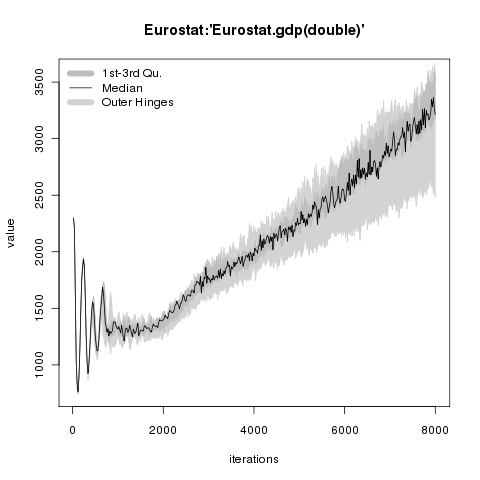
\includegraphics[width=8cm]{./transient/tax_0.08/Eurostat-gdp.png}
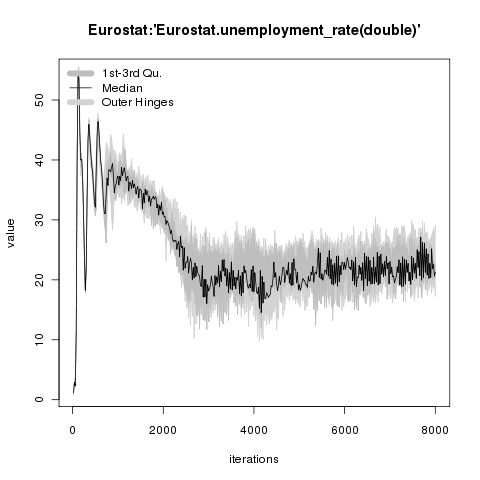
\includegraphics[width=8cm]{./transient/tax_0.08/Eurostat-unemployment_rate.png}\\
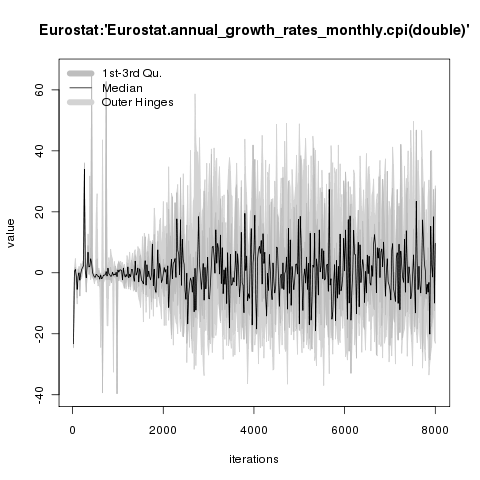
\includegraphics[width=8cm]{./transient/tax_0.08/Eurostat-cpi.png}
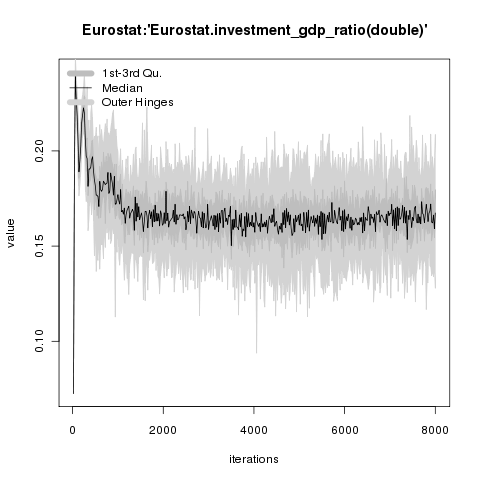
\includegraphics[width=8cm]{./transient/tax_0.08/Eurostat-investment_gdp_ratio.png}
\end{minipage}
\caption{Time series plots for 20 batch runs. GDP, unemployment rate, inflation rate and investment/GDP ratio.}
\label{Figure: transient time}
\end{figure}

%\subsubsection*{Distribution across batch runs}

\begin{figure}[ht!]
\centering\leavevmode
\begin{minipage}{17cm}
\centering\leavevmode
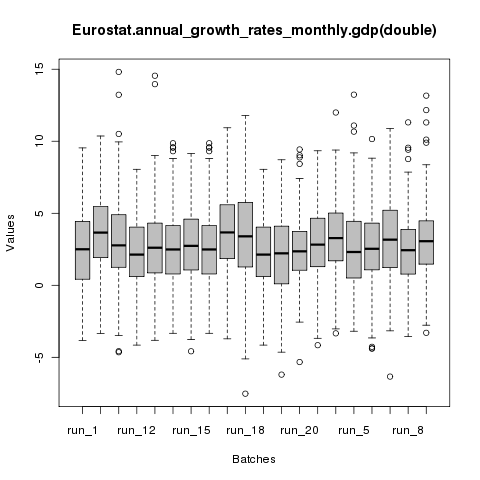
\includegraphics[width=8cm]{./benchmark_plots/Eurostat-annual_growth_rates_monthly-gdp-batches.png}
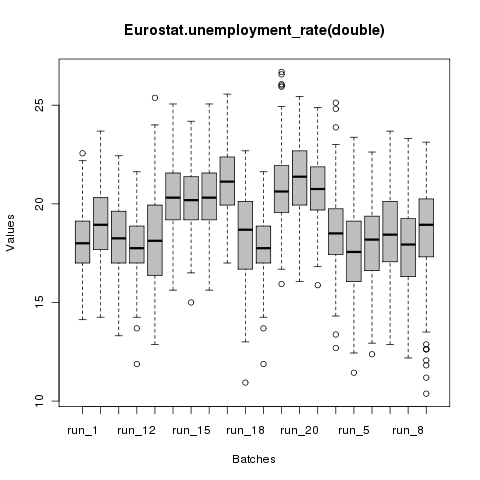
\includegraphics[width=8cm]{./benchmark_plots/Eurostat-unemployment_rate-batches.png}\\
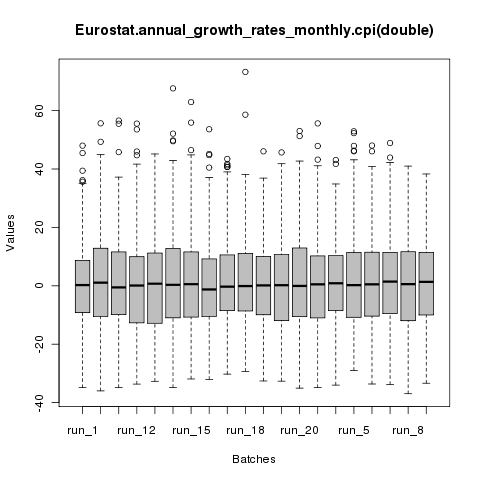
\includegraphics[width=8cm]{./benchmark_plots/Eurostat-cpi-batches.png}
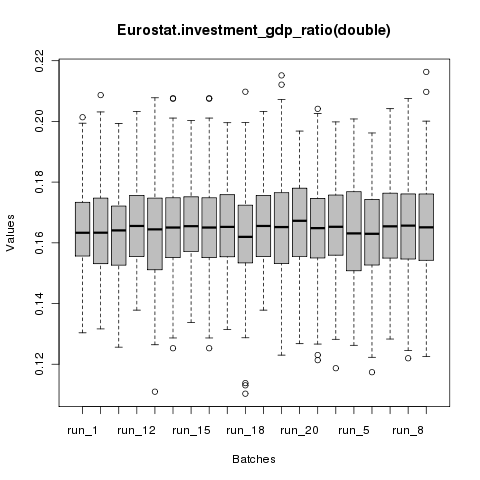
\includegraphics[width=8cm]{./benchmark_plots/Eurostat-investment_gdp_ratio-batches.png}
\end{minipage}
\caption{Box plots for separate runs of GDP, unemployment rate, inflation rate and investment/GDP ratio.}
\label{Figure: run batch}
\end{figure}

%\subsection{Approach to Benchmarking}
Our approach to benchmarking has been incremental: starting from this simplest model and then gradually increasing complexity. The benchmarks run so far are part of the assessment of the current parallel implementation. They also serve as a useful way of ensuring that FLAME and its generate applications are portable over and wide range of hardware and operating systems. 

\begin{table}[ht]
	\centering
		\begin{tabular}{l|ccc}
		Model 				& Agents & Messages & Populations 		\\\hline
		Circles  			&   1    &   1      &  2000 10$^5$   	\\
		C@S  					&   3    &   9      &  12,400 124,000 \\
		Labour Market &   4    &   10     &  11,011 110,101 \\ 
		Bielefeld	    &   4    &   29     &  4130 43100     \\\hline
		\end{tabular}
\end{table}

The starting populations have been generated using the initial population generator developed by STFC. The ratio of agents numbers in each population was retained from the original values.

Each benchmark has been on a variety of HPC systems available to STFC using a range of process numbers: 4 9 16 32 49 64 81 and 100. The results presented show how the lapsed time per iteration varies with number of processors. In these experiments a round-robin initial distribution has been used.
\subsection{The Circles Model}
The Circles agent is very simple. It has a position in two-dimensional space and a radius of influence. Each agent will react to its neighbours within its interaction radius repulsively. So given a sufficient simulation time the initial distribution of agents will tend to a field of uniformly spaced agents.

The description of the agent is given as a example of XMML in the sections above. Each agent has $x$, $y$, $fx$, $fy$ and $radius$ in its memory and has three states: outputdata, inputdata and move. The agents communicate via a single message board, $location$, which holds the agent $id$ and position.

The Circles problem is very simple but allows us an initial assessment of the performance of the parallelisation within FLAME. The simulation was started with a populations of $10^6$  agents and experiments performed using from 4 to 100 processors. The averaged results are shown in Table~\ref{tab:ExecutionTimesForCircles} and Figure~\ref{fig:Circles-graph}.
\subsection{The C@S Model}
The C@S model was the first economic model to be implemented in FLAME by the EURACE Project.  It is based on work detailed in Delli Gatti \textsl{et al.} \cite{Delli Gatti} where an economy is populated by a finite number of \textsl{firms}, \textsl{workers}/\textsl{consumers} and \textsl{banks}. The acronym C@S stands for \textsl{Complex Adaptive Trivial System}.

This provides an initial economic model for testing FLAME. The EURACE version of C@S contains models for consumption goods, labour services and credit services. The population is a mix of agents: \textsl{Malls}, \textsl{Firms} and \textsl{People}. Each of these has different states and communicates with other agents in the population through 9 message types.

As the agents in the C@S Model have some positional/location data and the communication is localised, the initial distribution of agents to processors, as in the Circles Model, can be based on location. This helps reduce cross-processor communication.

The initial population contained: 20000 firms, 100000 people and 4000 malls (124000 agents in total).
\subsection{Initial Labour Market}
This model was first model based on the work of the EURACE project. The model represented a very simplified labour market. It contains four agent types and 10 message types.
\subsection{Bielefeld Labour Market}
This model was a refinement of the Initial Labour Market. Its also contained four agent types but with 27 message types.
\subsection{EURACE Models}
During the development of the EURACE Model a number of domain specific models have been developed. These models were then integrated into the EURACE Model. Three domain specific models were developed: Credit Market, Labour Market and Financial Market. Each of these and the combine EURACE Model are the major economic models developed by EURACE. As part of the development of FLAME these models have been used to test the FLAME application generation and the framework infrastructure. In particular they have been very useful in testing the parallel implementation of FLAME. Although the initial agent populations is these models are very small they do encapsulate the full range and complexity of the EURACE model and to that end they are a very useful testing resource.

\begin{table}[ht]
	\centering
		\begin{tabular}{l|ccc}
		Model & Agents & Messages & Population \\\hline
		Financial Market  &    4    &   6       &  1104          \\
		Labour Market   &   7     &    45      &   1236         \\
		Credit Market   &   3     &    12      &   110         \\ 
		EURACE Model    &   9     &    54       &  2029         \\\hline
		\end{tabular}
\end{table}

All these models have been successfully parsed, compile and executed in both serial and parallel on some of our target HPC machines.
\input{benchmarks-0.08}
%\begin{figure}[ht!]
\centering\leavevmode
\begin{minipage}{7.5cm}
\centering\leavevmode
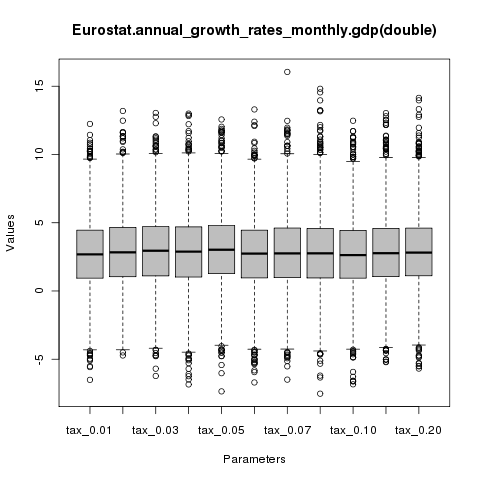
\includegraphics[width=6cm]{./batch/Eurostat-annual_growth_rates_monthly-gdp-scenarios.png}\\
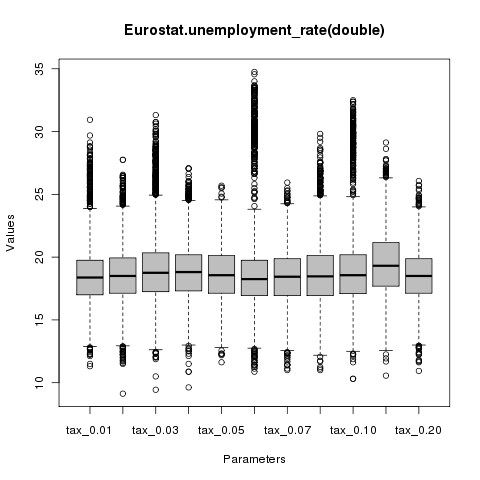
\includegraphics[width=6cm]{./batch/Eurostat-unemployment_rate-scenarios.png}\\
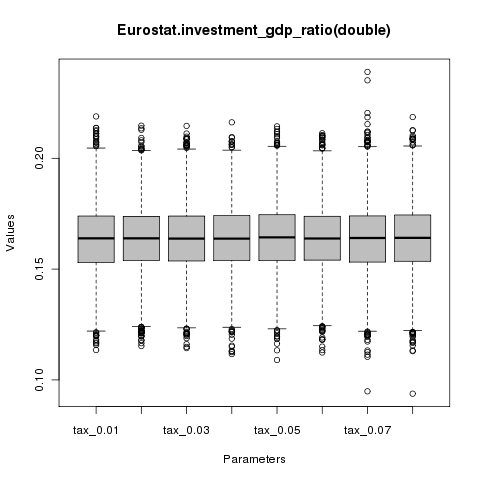
\includegraphics[width=6cm]{./batch/Eurostat-investment_gdp_ratio-scenarios.png}
\end{minipage}
\caption{Parameter sensitivity analysis for different tax rates of $0-8\%$ and $10,15,20\%$. Results are for $20$ batch runs over $4000$ periods (using periods $4001$ to $8000$).}
\label{Figure: scenarios}
\end{figure}


